\documentclass[11pt,a4paper]{article}

\usepackage[top=1.25cm,bottom=1.15cm,left=1.15cm,right=1.15cm]{geometry}
\usepackage[T1]{fontenc}
\usepackage[utf8]{inputenc}
\usepackage{lmodern}
\usepackage{enumitem}
\usepackage[hidelinks]{hyperref}
\usepackage{xcolor}
\usepackage{titlesec}
\usepackage{microtype}
\usepackage{tabularx}
\usepackage{fontawesome5}
\usepackage{pagecolor}

\usepackage{helvet}
\renewcommand{\familydefault}{\sfdefault}

\pagestyle{empty}
\setlength{\parindent}{0pt}
\setlength{\parskip}{4pt}
\hfuzz=3pt
\setlist[itemize]{leftmargin=*, topsep=1pt, itemsep=1pt}

\definecolor{heading}{RGB}{25,25,25}
\definecolor{timelineblue}{RGB}{30,58,95}
\definecolor{timelinegray}{RGB}{80,80,80}

\definecolor{pagebg}{RGB}{241,241,244}
\definecolor{cardbg}{RGB}{255,255,255}
\pagecolor{pagebg}

\titleformat{\section}{\large\bfseries\color{heading}}{}{0pt}{}[\vspace{-4pt}\hrule\vspace{4pt}]

\usepackage{tikz}
\usetikzlibrary{positioning}

\newcommand{\projectcard}[4]{
\noindent
\begin{tikzpicture}
\node[
    text width=0.96\textwidth,
    fill=cardbg,
    draw=timelinegray!25,
    rounded corners=3pt,
    inner sep=6pt,
    align=left
] (box) {
\begin{tabularx}{0.96\textwidth}{@{}p{1.05cm}@{\hspace{0.3cm}}X@{}}
{\LARGE\color{timelineblue}#1} &
\begin{minipage}[t]{\linewidth}
{\normalsize\textbf{#2}}\\[2pt]
{\footnotesize #3}
\end{minipage}
\end{tabularx}
};

\node[
    anchor=south east,
    fill=gray!8,
    draw=timelinegray!20,
    rounded corners=2pt,
    inner xsep=5pt,
    inner ysep=2pt
] at ([xshift=-6pt,yshift=6pt]box.south east) {
    {\tiny #4}
};

\end{tikzpicture}
\vspace{3pt}
}

\begin{document}

\noindent\rlap{%
\begin{tikzpicture}[remember picture,overlay]
\node[
    anchor=south,
    yshift=0.35cm,
    text width=17.9cm,
    fill=cardbg,
    draw=timelineblue!35,
    rounded corners=5pt,
    inner sep=8pt
] at (current page.south) {
{\scriptsize
{\small\bfseries\color{timelineblue}
\faCogs\ SKILLS
}

{\color{timelineblue!40}\rule{\linewidth}{0.4pt}}

\vspace{3pt}
\begin{tabularx}{17.7cm}{@{}X X X X X@{}}
\textbf{\color{timelineblue}Android Development} &
\textbf{\color{timelineblue}Architecture} &
\textbf{\color{timelineblue}Product Engineering} &
\textbf{\color{timelineblue}Quality} &
\textbf{\color{timelineblue}Additional Systems} \\[3pt]

Kotlin &
MVVM &
Feature Development &
Automated Testing &
Android Enterprise \\

Android SDK &
Clean Architecture &
Prototyping &
Debugging &
Device Owner \\

Coroutines &
Reusable Components &
UI Implementation &
Documentation &
Python / FastAPI \\

Flow &
Modular Design &
Release Delivery &
Release Validation &
PowerShell / AD \\

REST APIs &
Separation of Concerns &
Multi-device Support &
Maintainability &
Kerberos \\
\end{tabularx}
}
};
\end{tikzpicture}%
}
\begin{tabularx}{\textwidth}{@{}X r@{}}
    {\LARGE \textbf{Daniele Della Cioppa}} &
    \href{https://github.com/danieledellacioppa}{\Large \faGithub\ GitHub} \\
    {\normalsize Android Software Engineer --- Kotlin, Product Development \& Mobile Platforms} &
    \href{https://www.linkedin.com/in/daniele-della-cioppa-41b062115/}{\Large \faLinkedin\ LinkedIn} \\
    London, UK & \\
\end{tabularx}

\smallskip

\footnotesize{
Android Software Engineer with 5+ years of professional experience building Kotlin Android applications and mobile platform features across the full feature lifecycle, from requirements analysis and prototyping through implementation, testing, release and ongoing improvement. I develop maintainable Android software using MVVM, Clean Architecture, coroutines, Flow and REST APIs, with a focus on reliability, reusable components and clear separation of responsibilities. My work includes user-facing launcher, kiosk, whiteboard, digital signage, casting, provisioning and remote-control experiences across Android devices, large screens, managed-device platforms, hardware generations and vendor-specific integrations. I collaborate with technical leadership, operations, firmware, vendors and customer-facing colleagues to turn complex requirements into practical product solutions. Complementary systems experience includes Python/FastAPI services, PowerShell, Active Directory and Kerberos/SPNEGO automation.

}


\section*{Work Experience}

\renewcommand{\arraystretch}{1.08}
\begin{tabularx}{\textwidth}{>{\raggedleft\arraybackslash}p{2.4cm} !{\color{timelinegray}\vrule width 0.8pt} >{\raggedright\arraybackslash}X}
\textbf{\color{timelineblue}\shortstack[r]{2025--2026\\Current}} &
\textbf{Software Developer --- Akhter Computers}\\
& {\small\color{timelinegray}\textbf{Android Product Development, Mobile Platforms \& Cross-Platform Systems}}
\par{\footnotesize
\begin{itemize}
    \item Developed Kotlin-based Android applications and user-facing platform features from initial requirements through implementation, debugging, validation, release and follow-up improvements.
    \item Prototyped and iterated interactions for launcher, kiosk, whiteboard, floating annotation, casting, pairing, provisioning, remote-control and device-configuration experiences.
    \item Supported Android applications across multiple hardware generations, Android versions, large-screen devices and vendor-specific device platforms.
    \item Integrated Android applications with REST APIs, backend services and cross-platform Windows/Linux components for command reporting, content delivery, remote management and controlled updates.
    \item Worked with technical leadership, operations, firmware teams, vendors and customer-facing colleagues to refine requirements, validate releases and resolve product issues across devices.
    \item Contributed additional backend and infrastructure experience using Python, FastAPI, PowerShell, Active Directory, Kerberos/SPNEGO, SMB and Group Policy automation.
\end{itemize}} \\[3pt]

\textbf{\color{timelineblue}2024--2025} &
\textbf{Android System Developer --- Distributed Device Systems}\\
& {\footnotesize\color{timelinegray}
\begin{itemize}
    \item Delivered Kotlin Android features for distributed digital-signage and device-synchronisation systems, including user-visible content playback, status reporting and remote operations.
    \item Built reusable Android components around MVVM and Clean Architecture boundaries, separating UI, networking, persistence, orchestration and device-control responsibilities.
    \item Integrated Android clients with REST APIs and Linux-backed services for content delivery, command/status reporting, update orchestration and release validation.
    \item Used Kotlin coroutines and Flow for asynchronous device state, background synchronisation, network calls and resilience during intermittent connectivity.
    \item Improved component boundaries, compatibility checks and release/update paths to support maintainability across managed signage devices.
\end{itemize}} \\[2pt]

\textbf{\color{timelineblue}2023--2024} &
\textbf{Android System Developer --- Remote MDM \& Update Infrastructure}\\
& {\footnotesize\color{timelinegray}
\begin{itemize}
    \item Developed reusable Kotlin Android platform capabilities for provisioning, application delivery, state reporting, command handling and local device workflows.
    \item Built Android Enterprise Device Owner and Device Policy Manager integrations for kiosk behaviour, managed configuration and controlled user/device actions.
    \item Implemented APK delivery and update workflows with signature/hash verification, controlled rollout behaviour and release validation.
    \item Supported Gradle builds, CI/CD release packaging, automated validation and debugging across Android clients, Linux-backed services and operational tooling.
\end{itemize}} \\[2pt]

\textbf{\color{timelineblue}2021--2023} &
\textbf{Software Development Apprenticeship}\\
& {\scriptsize\color{timelinegray}
\begin{itemize}
    \item Contributed to Android and IoT projects involving API integration, telemetry, debugging, automated testing, monitoring and customer-facing operational support.
\end{itemize}}
\end{tabularx}

\clearpage
\section*{Main Projects}

\projectcard
{\faMobile}
{Android Launcher, Kiosk \& Collaboration Features}
{Developed and prototyped Kotlin Android user-facing features for launcher, kiosk, whiteboard, floating annotation, pairing, remote-control and device-configuration workflows across large-screen and managed-device platforms.}
{Kotlin / UI}

\projectcard
{\faTv}
{Distributed Android Digital Signage Platform}
{Built Kotlin Android digital-signage and synchronisation capabilities for content playback, REST API integration, content delivery, remote operations, Gradle packaging and local-first resilience.}
{Kotlin / REST}

\projectcard
{\faDesktop}
{Cross-Platform Screen Casting R\&D}
{Prototyped Android and Windows screen-casting paths, comparing MediaProjection apps, Windows sender tooling, PhairPlay-based Android receiver work, AirPlay research, Miracast/WFD investigation and WebRTC receiver/sender experiments.}
{Android / WebRTC}

\projectcard
{\faLock}
{Android Device Management \& Kiosk Platform}
{Developed Android platform capabilities around Device Owner provisioning, Device Policy Manager controls, kiosk behaviour, state reporting, command handling, controlled APK updates and release checks.}
{Device Owner}


\end{document}
